\documentclass{article}
\usepackage[utf8]{inputenc}

\usepackage[dvipsnames]{xcolor}
% \usepackage[altpo]{backnaur}

\usepackage{
  amsmath, amssymb, amsthm, thmtools, thm-restate, tikz, graphicx,
  hyperref, cleveref, comment, expl3, xparse, ebproof, enumitem, stmaryrd,
  enumitem, verbatim, todonotes, xargs, url, mathtools, mathrsfs, xfrac, cite,
  setspace, titlesec, bbm, dirtytalk, fancyhdr, esvect, tikz, listings,
  % simplebnf,
  naive-ebnf
}

% \RenewDocumentCommand{\bnfexpr}{m}{$\langle \texttt{#1} \rangle$}

% \newcommand{\nonterminal}[1]{
%   $\langle \text{#1} \rangle$
% } 

\lstset{basicstyle=\small\ttfamily}

\crefname{lstlisting}{listing}{listings}
\Crefname{lstlisting}{Listing}{Listings}

\usetikzlibrary{shapes.geometric, arrows}

\newcommandx{\mygather}[3][1=1ex, 2=\normalsize]{
  \begin{spreadlines}{#1}
    {#2
      \begin{gather*}
        #3
      \end{gather*}
    }%
  \end{spreadlines}
}

\newcommandx{\myenumerate}[2][1=1ex]{
  \begin{enumerate}
    \setlength \itemsep{#1}
    #2
  \end{enumerate}
}

\newcommandx{\myitemize}[2][1=1ex]{
  \begin{itemize}
    \setlength \itemsep{#1}
    #2
  \end{itemize}
}

\newcommandx{\myalign}[3][1=1ex, 2=\normalsize]{
  \begin{spreadlines}{#1}
    {#2
    \begin{align*}
      #3
    \end{align*}
    }%
  \end{spreadlines}
}

\DeclareMathOperator{\Boolean}{\mathtt{Boolean}}
\DeclareMathOperator{\Class}{\mathtt{Class}}
\DeclareMathOperator{\Number}{\mathtt{Number}}
\DeclareMathOperator{\Object}{\mathtt{Object}}

\DeclareMathOperator{\decl}{decl}

\DeclareMathOperator{\Pre}{Pre}
\DeclareMathOperator{\Post}{Post}

\DeclareMathOperator{\true}{\mathtt{true}}
\DeclareMathOperator{\false}{\mathtt{false}}

\DeclareMathOperator{\dom}{dom}
\DeclareMathOperator{\N}{\mathbb{N}}

\newcommandx{\set}[2]{
  \{#1 \, | \, #2\}
}

\newcommandx{\mcrl}{\texttt{mcrl2}}

\newcommandx{\class}[2]{
    \texttt{class } #1 \, \{ #2 \}
}

\newcommandx{\classextends}[3]{
    \texttt{class } #1 \texttt{ extends } #2 \, \{ #3 \}
}

\newcommandx{\pair}[2]{
    (#1, \, #2)
}

\newcommandx{\jdgmt}[3][1=\Gamma, 2=\Delta]{
    #1; \, #2 \vdash #3
}

\newcommandx{\subtypejdgmt}[2]{
   #1 \leq_\Delta #2 
}

% https://tex.stackexchange.com/questions/9796/how-to-add-todo-notes
\newcommandx{\info}[2][1=] {
  \vspace{5mm}
  \todo[inline, linecolor=OliveGreen,backgroundcolor=OliveGreen!25,bordercolor=OliveGreen,#1]{#2}
  \vspace{5mm}
}

\newcommandx{\inlinetodo}[1]{
  \info{
    \textbf{TODO}

    #1
  }
}

% Title information
\title{Formalizing a simple loan agreement in L4 and Maude}
\author{
  Joe Watt
  \and
  Oliver Goodenough
}
% \date{June 2022}

\begin{document}

% Title and table of contents.
\maketitle

\info{
  This is a work in progress.
}

\tableofcontents

\newpage

% Main body.

\section{Introduction}

% \inlinetodo{
%   Write a better intro and provide more background on
%   \cite{contract_as_automaton}.
% }
% \inlinetodo{
%   Write a proper introduction to the original work on formalizing the simple
%   loan agreement as a DFA.
% }

% In \cite{contract_as_automaton}, Flood and Goodenough propose that many financial
% contracts are inherently computational in nature.
% They argue that the computational structure of many such contracts
% can be formalized via deterministic finite automata (DFAs), with states
% representing various situations.
% % like ``borrower default'' and ``payment due''.
% Transitions between these states then correspond to events triggering a change
% in these situations.
% This is demonstrated using a simple loan agreement
% \cite[Table 1]{contract_as_automaton}, which they formalize
% directly as a DFA.

In \cite{contract_as_automaton}, Flood \& Goodenough propose that many
financial contracts are inherently computational in nature.
They argue that the computational structure of many such contracts can be
formalized via deterministic finite automata (DFAs), with states representing
various situations.
Transitions between these states then correspond to events triggering a change
in these situations.
This is demonstrated using a simple loan agreement \cite{contract_as_automaton},
which they formalize directly as a DFA.

While the DFA approach is a useful and important proof of concept, as the authors
themselves recognize, there are some limitations with such a formalism, perhaps
the most apparent being that the manual encoding of a contract as a DFA is a
laborious process, and one that in itself does not produce a machine executable
result.

Our first demonstration in this paper is using the L4 language being developed
at the Singapore Management University (SMU)
to represent the bargain described by Flood \& Goodenough
\cite{contract_as_automaton}.
Through this, we show how L4 addresses some shortcomings of the DFA
formalization.

Next, we  discuss how we implemented an execution engine that allows us to
execute contracts written in L4.
For this, we designed a Structural Operational Semantics (SOS)
\todo{Cite Plotkin's seminal paper} for L4, giving us a mathematical
description of the execution behavior of contracts.
To make this executable, we implemented this mathematical description in
the Maude language, which in turn enables us to generate interactive
visualizations of the resulting transition system.
 

\section{Shortcomings of the DFA formalization}
As aforementioned, DFAs quickly become cumbersome to work with directly when
the contracts we are trying to encode grow larger.
One source of complexity arises from the fact that the DFA is a low level
computational formalism that is arguably far removed from our intuitive
understanding of a contract.
While we can easily encode real-world events as transitions in a DFA, as done
in \cite{contract_as_automaton}, some legal traditions reason about and specify
contracts in terms of normative requirements that need to be fulfilled by
various actors \cite{normative_compliance_guido}.
The authors of this paper, representing different traditions, do not entirely
agree on this point, but it remains true that a DFA is a relatively
mechanistic chain of event and consequence, and is not adept at normative
representation.

Contracts also frequently embody some notion of time and deadline.
These are examples of domain-specific concepts which are an integral
part of contract drafting.
Unfortunately, DFAs have no primitive notion of these, so that these must all
be encoded manually, with the passage of time reflected as an achieved event,
in a manner that is perhaps unnatural to many.

Another source of complexity is the state explosion problem.
Complex contracts have large DFA representations and are thus impractical for
humans to specify manually at scale.
Observe that a simplified visual representation of the automaton
\cite[Fig. 1]{contract_as_automaton}
corresponding to this simple contract already contains more than 20 states and
40 transitions.

% Consequently, a more practical formalism should provide mechanisms like
% global variables and arithmetic operations.

% Such an issue could be addressed by a formalism that is more sophisticated than
% a DFA, something that allows for global variables, which can be updated at
% runtime.

% Ideally, we would like to be able to collapse these into a single subgraph
% corresponding to the``accelerated repayments'' phase of the contract.
% However, this is not possible here as both accelerated repayment stages as in
% the 

% Likewise, the transitions between them are similar as well, with the only
% difference being the 

% % verbose duplication of states along the main ``happy path''.

% What we mean instead is that there are similarly named states whose subgraphs
% have similar structure.
% These include the 2 main repayment stages along this path, given by the
% ``Payment\dots accruing'' states.
% Each of the subgraphs rooted at these nodes has a similar structure, with
% borrower default events giving rise to transitions to the unhappy paths.
% These in turn also have similar structure, with similar
% ``Payment\dots accelerating'' and ``Crisis\dots'' states.
% The only difference between the transitions between these states is

One of the main causes of this is the concurrent interleaving of real
world events.
By this, we mean that many real world events can occur in any order (including
at the same time) and
perhaps for the sake of simplicity, this has not been accounted for in the DFA
formalization.
As an example of such a scenario, consider the following.
On May 31, 2015, the day before payment 1 is due, the borrower defaults on his
representations and warranties.
On the next day, when payment 1 becomes due, the borrower diligently
repays that payment.
One day later, on June 2, 2015, the lender notifies the borrower of his
earlier default, which does not get cured after another 2 days.
Now all outstanding payments become accelerated, and the borrower pays off
the remaining amount of \$525 in time, causing the contract to terminate.
This sequence of events, when viewed as a word over the event alphabet, is
unfortunately not accepted by the automaton.

Closer inspection of the DFA suggests that there is an
implicit assumption being made that once an event of default occurs,
the borrower will be notified by the lender soon after, with no other events
like payments occurring in between.

More formally, it is assumed that the default and notification events occur
within the same atomic step.
Splitting this up into separate events would increase the number of states in
the DFA, especially if we account for concurrency.
In fairness, Flood and Goodenough understood some of these limits, and specified
in \cite{contract_as_automaton}[Section 6] of their model agreement that:
``In the event of multiple events of default, the first to occur shall take
precedence for the purposes of specifying outcomes under this agreement''.
This provision goes some way toward resolving competing defaults by the
expedient of mandating that later events will simply be disregarded.

% Workspace
% \info{
%   Other weaknesses to mention:

%   Representation of time and deadlines.
%   Not handled well by the DFA, but is an important notion that exists in L4.
%   These are translated to Maude.

%   No explicit notion of deontics, which is important to humans because that's
%   what people are used to reasoning about and normative language shows up
%   everywhere in legal drafting.
%   In L4, we have a notion of deontics, though not quite the same as deontic logic.
%   We have an operational interpretation that is made precise by the translation
%   to Maude.

%   The focus here is that a friendly-to-use language should provide appropriate
%   abstractions corresponding to concepts found in the application domain.
%   For the legal domain, these include the notions of rules, actors, events, 
%   deadlines and deontics.
%   Another reason for modelling these explicitly is to be able to achieve a
%   nice correspondence (more technically an isomorphism) with legal texts that
%   are drafted in natural language.
% }

% Old not useful
% It should be noted here that this only poses problems in the manual encoding
% of a contract, by hand, as a DFA.
% For the purposes of automated reasoning as in the field of 
% \textit{formal verification}, model checking tools like UPPAAL
% \todo{cite properly here}
% are able to automatically analyze automata comprising thousands of states.

% Therefore, we argue that this evinces that accurately
% encoding contracts as a DFA directly is too laborious and difficult,
% even for a contract as simple as the one presented in
% \cite[Fig 1.]{contract_as_automaton}.
% In our view, a more practical formalism should sit at a higher-level than a DFA,
% providing mechanisms for tackling these 2 issues.
% Firstly, it should provide global variables, or at least, some way of encoding
% global state.
% There should also be operations that allow us to retrieve and update the global
% state.
% Secondly, it should be able to conveniently accommodate the concurrency
% inherent in the real world.
% Consequently, we believe that a practical formalism for encoding contracts
% should be something higher-level than a DFA, one that can conveniently
% accommodate the concurrency inherent in the real world.
% Maudeetter still if the formalism comes with tools that allow us to compile down
% to something like automata for visualization and automated reasoning.

% However, it should be noted that for the purposes of visualization and
% automated reasoning in the sense of \textit{formal verification}, DFAs are a
% suitable choice of formalism.
% Indeed, tools such as UPPAAL \todo{list more tools and cite properly} are able to
% efficiently simulate and analyze automata with thousands of states.
% In fact, these tools rely on analyzing \textit{labelled transition systems},
% generalizations of nondeterministic finite automata (NFA) that allow for
% infinitely \footnote{Possibly uncountably} many states and transitions.

\section{The L4 approach}
The L4 language for encoding legal texts is being developed at SMU which
addresses some of these shortcomings.
% At CCLAW, we are developing one such domain specific language (DSL) for
% specifying legal contracts, called L4, which aims to address some of these
% issues.
As described by its developers,
``L4 is a domain-specific specification language that facilitates semantically
rigorous formalization of legal expressions found in legislation and
contracts.''
(Mahajan, Strecker \& Wong. 2022)
\todo{cite properly}

Its core approach utilizes a natural language-based structure and syntax which
allows the detailed, if artificially structured, expression of the obligations
and consequences that need to be set out in a legal specification.
The programming language recognizes the logic embedded in these statements and
then allows that logic to be represented in a number of different execution
software approaches.
(Id)
\todo{cite properly}
It is capable of representing both the private bargains of contract and the
public prohibitions and requirements of statutes and regulations.
Additional background on L4 and its applications is available at \_ \todo{Cite}. 

% Along with L4, the developers are also developing an accompanying toolset
% which can be used to visualize and analyze contracts written in L4.
% Here we first give an introduction to our project and the L4 DSL that
% we are developing, before discussing our formalization of the loan agreement in
% the next section.

As described in
\todo{Cite WAICOM 2022 and PROLALA 2022 papers},
L4, as with LegalRuleML \todo{Cite LegalRuleML}, distinguishes between two
kinds of rules, namely constitutive and regulative (or prescriptive) rules.
The former encodes static decision logic, similar to Prolog-style
\textit{if-then} rules.
\todo{Insert example, like the one in PROLALA paper}

Our focus in this work is on the latter, namely regulative rules, which concern
the norms in a legal text.
These are a central component in the computational structure of contracts like
the loan agreement.
They govern under which conditions an actor is allowed,
permitted or prohibited from performing an action, as well as the consequences
of fulfilling and violating them.

% Such consequences include new norms that come into effect, like
% contrary-to-duty ones \todo{Cite something about CTD norms} which are triggered
% upon the violation of other norms.

While deontic logic approaches have been popular,
\todo{Cite appropriately}
our approach to regulative rules in L4 is closer in spirit to
\cite{real_time_contract_automata, normative_diags_diogo},
\todo{Cite the Maude paper as well, and any others that are relevant}
in that our treatment of the rules is operational in nature, grounded in the
mathematical framework of SOS.
This yields a state transition system, similar in spirit to the DFA found in
the work of Flood \& Goodenough \cite{contract_as_automaton}.
% Our operational treatment of these regulative rules, or more formally an
% operational semantics, is implemented in the Maude language.
% This is used to construct DFA visualizations of contracts specified in L4,
% as well as simulate executions and perform various forms of analysis.

\subsection{Syntax of regulative rules}
Here we describe the natural-language like syntax for specifying regulative
rules in L4, as well as a brief discussion of the relevant domain specific
concepts.
A more detailed discussion with some examples will be provided in the following
section, in the context of our encoding of the loan agreement.

Regulative rules in L4 have the following form, with special keywords given
in all-caps:
\begin{lstlisting}
  RULE rule name
  PARTY actor
  deontic
  deadline
  [ DO ] action
  [ HENCE hence_0 AND ... AND hence_n ]
  [ LEST lest_0 AND ... AND lest_n ]
\end{lstlisting}

Note that the \texttt{deadline}, \texttt{DO} keyword, as well as the
\texttt{HENCE} and \texttt{CLAUSES} are optional.
We also allow for some permutations of the \texttt{deontic}, \texttt{deadline}
and \texttt{action} clauses.

Each clause in the above rule corresponds to the following
domain concepts that we have identified:
\begin{itemize}
  \item \texttt{actor}
  \item \texttt{action}

  Actors and actions are currently plain strings with no special meaning
  attached to them.
  
  \item \texttt{deontic}

  There are 3 kinds of deontics:
  \begin{itemize}
    \item \texttt{MUST}: Achievement obligation
    \item \texttt{MAY}: Permission
    \item \texttt{SHANT}: Prohibition
  \end{itemize}

  \item \texttt{deadline}

  This can take the form:
  \begin{itemize}
    \item \texttt{WITHIN} $n$ \texttt{DAY}
    \item \texttt{ON} $n$ \texttt{DAY}
  \end{itemize}

  These are relative to the time when the rule comes into effect and
  \texttt{WITHIN} $n$ \texttt{DAY} indicates that the action may occur at any
  time within the next $n$ days, while \texttt{ON} $n$ \texttt{DAY} means that it
  may only occur on the $n$-th day itself.

  Note that we currently do not support weeks, months, years as well as fixed
  dates, though we intend to add support for these in the future.
  Also, all rule are currently required to include a deadline.
  We intend to relax this in the future.

  \item \texttt{hence\_i} (resp \texttt{lest\_i})

  \texttt{hence\_i} (resp \texttt{lest\_i}) are rule names denoting rules that
  are triggered when the obligation or prohibition is fulfilled (resp violated).
  We identify the fulfillment of an obligation with whether the actor performed
  the prescribed action within the deadline, and violation is identified with
  the deadline passing before the actor performs the action.

  Fulfillment and violation for prohibitions are defined symmetrically.

  % \todo{Looks a bit terse, break it up and explain more}
  % With this, one can encode \textit{contrary-to-duty} rules as
  % \texttt{lest\_i} rules that appear in the \texttt{LEST} clause, as these come
  % into effect on violation of an obligation/prohibition.

  In the case of permissions, the \texttt{hence\_i} are triggered when the
  permission is exercised, and the \texttt{lest\_i} are triggered when it
  is not exercised by the deadline. 
\end{itemize}

For instance, consider an obligation of the form
\begin{lstlisting}
    RULE rule
    PARTY actor
    MUST DO action
    WITHIN 3 DAY
    HENCE hence
    LEST lest0 AND lest1
\end{lstlisting}

% The idea is that when such a rule is triggered, we start a timer to keep track
% of its deadline.
% For the above rule, we start a timer which begins counting down 1 day at a time,
% from 3 days.
If \texttt{actor} performs \texttt{action} on days 0, 1 or 2, we deem the
obligation to have been fulfilled, and the timer is stopped.
In this case, the rule named \texttt{hence} now takes effect and a new timer
begins.
If instead, 3 days pass without the actor performing the action, we deem the
rule to have been violated.
Now, the two rules, \texttt{lest0} and \texttt{lest1}, in the
\texttt{LEST} clause are triggered.

% Note that when rules with missing deadlines are triggered, they are treated as
% having a timer with an infinite value, which means that obligations with no
% deadline can never be violated.

% Regulative rules on the other hand, concern norms in a legal text, and are
% traditionally expressed in normative language, utilizing deontic operators
% like must, may and shant.

% Our focus here is on these regulative rules
% which we argue can be seen as
% defining a transition system -- a generalization of finite state automata,

% Here, we adopt the view that these regulative rules define

% we ascribe an operational interpretation to these rules,
% similar

% consider regulative rules as

% Our focus here is on regulative rules and our view is that contracts can be
% seen as a behaviour

% structure of a legal
% text, and can be viewed as defining a transition system -- a generalization
% of nondeterministic automata.

% \inlinetodo{
%   Talk about constitutive and regulative rules.

%   Constitutive rules as statics, semantics is arguably straightforward, namely
%   some first order defeasible logic.
%   Can be formalized using Prolog.

%   Regulative rules as dynamics, trickier semantics, is the focus of this paper.
%   Will show how the loan agreement is modelled using these.

%   Give an example of a regulative rule found in the loan agreement to
%   demonstrate the syntax. Then use this example to highlight domain specific
%   concepts.
%   Read \cite{normative_diags_diogo,real_time_contract_automata} 
%   and highlight similarities with them.
% }

% As mentioned earlier, we believe that a friendly to use language for specifying
% legal contracts should be situated at a higher level of abstraction than that
% of automata, closer to the application domain.

% \info{
%   Workspace:

%   It comes with a concurrent model of computation (this is made precise
%   by the translation to Maude) which allows for arbitrary interleaving of events.

%   It is also friendly to use, containing ontological
%   concepts from the legal domain that people are used to thinking about and
%   working with.

%   Discuss the precise roles of these concepts and how the execution of a
%   contract can be viewed abstractly as a process that arises from the interaction
%   between them.

%   Mention that the precise operational interpretation of rules in L4 is tightly
%   linked to the translation in Maude and this was heavily inspired by
%   \cite{symboleo_model_checking_contracts,eventb_data_sharing_agreements}.

%   We view a rule as a wrapper around an event, a deontic (ie permission,
%   obligation or prohibition) and an actor.
%   Our treatment of deontics accounts for the notion of \textit{compensability},
%   and is based on \cite{normative_compliance_guido}.

%   Note that the difference is that instead of reasoning about deontics using
%   deontic logic, we provide an \textit{operational} interpretation for them.
% }

\subsection{The loan agreement in L4}
(TODO:
\href{
  https://docs.google.com/spreadsheets/d/1_k17mzk2hTyPY2egbEVqXzr8uYAdi6BVqeMYdBxKB_I/edit#gid=864296175
}{Add link})

It should be mentioned that our encoding of the loan agreement is an
approximation of the
one in the original paper \cite{contract_as_automaton} as we currently lack
certain features like fixed dates, which are used as deadlines in the original
contract.
To cope with this, we specify deadlines in terms of days relative to the
time the rule triggers, in place of dates.
Other limitations and inadequacies will be pointed out along the way.

% To operationalize a contract, we assume that the first rule at the top of an
% L4 encoding is the starting rule, which is triggered once we begin executing
% the contract.
The following rule is found at the beginning of our encoding of the loan
agreement.
We assume that the first rule in an L4 encoding is the starting rule which is
triggered at the beginning of the contract.

\begin{lstlisting}
  RULE Contract Commencement
  PARTY Borrower
  MAY WITHIN 1 DAY
  request funds
  HENCE Remit principal
\end{lstlisting}

This starting rule says that the actor, \texttt{Borrower},
may perform the \texttt{request principal} action any time from the time the
rule comes into effect up til 1 day later.
Note that for simplicity, we assume that permissions are one-off and are
used up once the action occurs, so that no repeated actions are allowed.
This assumption mirrors that of \cite{real_time_contract_automata}, in which
the author notes that one can also allow for permissions that may be exercised
more than once.
In the future, we hope to lift this restriction.

The \texttt{HENCE} clause is then used to indicate that if the permission is
exercised, then another rule called \texttt{Remit Principal} comes into effect.
The lack of a \texttt{LEST} clause indicates that no new rule is triggered
when the deadline passes without the permission being exercised.

The \texttt{Remit principal} rule is then expressed as follows:

\begin{lstlisting}
  RULE Remit principal		
  PARTY	Lender		
  MUST remit principal
       in the amount of 1000
       to Borrower
  WITHIN 1 DAY
  HENCE	Repayment
\end{lstlisting}

This obliges the lender to send the principal amount to the borrower once
the borrower has requested for it.
The \texttt{Repayment} rule defines the main body of the contract and comes
into effect when the \texttt{Remit principal} rule is fulfilled, ie when the
lender sends the principal to the borrower.
Note that L4 allows us to define a rule to be a conjunction of multiple rules
so that \texttt{Repayment} is defined as:

\begin{lstlisting}
        Repayment
  MEANS Repay in two halves
  AND   Avoid default
\end{lstlisting}

Triggering the composite \texttt{Repayment} rule then has the effect of
triggering the \texttt{Repay in two halves} and \texttt{Avoid default}
rules in parallel.
The former obliges the borrower to make the first repayment, followed by the
second, and the latter prohibits him from defaulting on representations and
warranties and so on.

It should be noted here that as in \_
\todo{
  cite one of Guido's papers that talks about contrary to duty norms and
  compensability
},
we distinguish between the violation of an obligation/prohibition, and the
violation of the contract as a whole.
Obligations and prohibitions like \texttt{Remit principal}, which do not have
a \texttt{LEST} clauses are assumed to be non-reparable.
This means that when this obligation is violated, we deem the contract to
have been breached by the lender.
Execution of the contract proceeds no further and to draw a parallel with
computer programs, we can view this as the contract (seen as a program)
throwing an unrecoverable exception during execution, causing it to terminate
in a breach state (ie crash).

% By viewing the, one can view the violation of a
% non-reparable obligations as throwing an unrecoverable error that terminates
% the execution of

In contrast, some rules, like the \texttt{Repay in two halves} obligation below,
have a nonempty \texttt{LEST} clause and so is deemed to be reparable, with
reparation mechanisms, or \textit{contrary-to-duty} rules
\todo{Cite a Guido paper on CTD norms and compensability}
, being encoded in the
\texttt{LEST} clause.
In this case, the violation of the rule results in the rules in the
\texttt{LEST} clause coming into effect, and the execution of the contract
continues, as opposed to terminating in a breach state.
Going back to the analogy with computer programs, one can view these
contrary-to-duty norms as exception handling mechanisms that activate in an
attempt to steer the execution of the contract back along the ``happy path''.

\begin{lstlisting}
  RULE Repay in two halves
  PARTY	Borrower
  MUST ON 10 DAY
  DO repay first half
     in the amount of 550
     to Lender
  HENCE	Repay second half
  LEST Notify borrower of default
\end{lstlisting}

In this rule, the \texttt{ON 10 DAY} deadline is used to mean that early
payments are not allowed, as in the original agreement.
While we could have chosen to encode 1 year as 365 days, due to the way in which
we handle time and deadlines under the hood, 365 days results in too large of a
transition system for our system to handle.
Thus, we have instead chosen a more modest deadline of 10 days.

The \texttt{Notify borrower of default} grants the lender permission to notify
the borrower and encodes the ``notice and cure'' reparation mechanism.
As noted in \cite{contract_as_automaton}, this indicates the
start of the reparation pathway, which gives the borrower a second chance, by
obliging him to cure his default.
Should he still not make amends, the execution of the contract has reached the
point of no return and no further second chances are given.
This is embodied by the activation of the
\texttt{Accelerate outstanding payments} obligation.

\begin{lstlisting}
  RULE Accelerate outstanding payments			
  PARTY Borrower
  MUST WITHIN 1 DAY	
  DO repay outstanding amount
     to Lender	
\end{lstlisting}

Unfortunately, while encoding this rule in L4, we realized that our
formalization does not faithfully implement the intuitive reading of its
corresponding natural language counterpart.
Intuitively, when the execution of the contract reaches this stage, no other
obligations are relevant anymore, like the \texttt{Avoid default} prohibition.
Consequently, one would like to be able to terminate
all existing obligations when this comes into effect.
While we would have liked to add support for this, we encountered various
complications and hence decided to leave this for future work.

\section{Operational semantics of Regulative Rules in L4}
% \info{
%   This section and the others after it are still heavily in progress.
% }

% Informally, the runtime state of a contract is either:
% \begin{enumerate}
%   \item
%   a set of rules that are active, along with their associated deadlines, which
%   we keep track of in the form of a timer that starts counting down one day at
%   a time, once the rule is triggered

%   Note that we say that the contract is fulfilled if this set is empty, ie if
%   there are no more active rules.

%   \item
% \end{enumerate}

In order to operationalize contracts for execution, we begin by formalizing a
semantics for regulative rules in L4 using the framework of Structural
Operational Semantics (SOS) \todo{Cite Plotkin}
originating from the field of programming language theory.

SOS is a mathematical framework which allows one to describe
transition systems in terms of states, called configurations, and transition
rules that describe how one state can transition to another.
These rules are expressed as logical inference rules of the form:

\begin{align*}
  \begin{prooftree}
    \hypo{H_1}
    \hypo{\dots}
    \hypo{H_n}
    \infer3{\smallstepsto{C}{E}{C'}}
  \end{prooftree}
\end{align*}

Here $\smallstepsto{C}{E}{C'}$ is known as a judgement form which expresses that
the configuration $C$ evaluates to $C'$ when an event $E$ occurs.
With this, the above transition rule is then read as saying that given a
configuration $C$, if all the hypotheses $H_i$ hold, then the event $E$ is
allowed to occur, and $C$ is allowed to transition to $C'$ when it does.

% \begin{lstlisting}
%     RULE rule
%     PARTY actor
%     MUST DO action
%     WITHIN 3 DAY
%     HENCE hence
%     LEST lest0 AND lest1
% \end{lstlisting}

% In the context of L4, the state of a configuration is either:
% \begin{enumerate}
%   \item Fulfilled 
% \end{enumerate}

Our configurations and transitions are parameterized over
a set of rules, called \texttt{Rule}.
Following timed transition systems, we define 2 kinds of events, namely action
events of the form \texttt{actor does action} and discrete tick events
indicating the passage of a day.
We then have the following transitions:

\begin{gather*}
  \begin{prooftree}
    \hypo{\text{if the \texttt{actor does action} event is allowed to occur in the configuration } C}
    \infer1[\text{action}]{C \overset{\texttt{actor does action}}{\longrightarrow} \delta_\text{action}(\texttt{actor does action}, \, C)}
  \end{prooftree}
  \\ \\
  \begin{prooftree}
    \infer0[\text{tick}]{C \overset{\text{tick}}{\longrightarrow} \delta_\text{tick}(C)}
  \end{prooftree}
\end{gather*}

where $\delta_\text{action}$ and $\delta_\text{tick}$ are transition functions
that compute the effect of action events and tick events on the current state
of the contract, by triggering rules found in the \texttt{HENCE} and
\texttt{LEST} clauses of a rule.
The use of the precondition for action transitions is to restrict actions so
that we can only take that transition when there is an active rule mentioning it.

More precisely, we say that an action event \texttt{actor does action} is allowed
to occur in a configuration $C$ if either:

\begin{itemize}
  \item
  There is a rule named $r$ with a deadline of the form
  \texttt{WITHIN n DAY}
  and $C$ contains an active rule instance of the form
  $\pair{r}{m}$ where $m \leq n$.

  \item
  There is a rule named $r$ with a deadline of the form
  \texttt{ON n DAY}
  and $C$ contains an active rule instance of the form
  $\pair{r}{0}$
\end{itemize}

Configurations $C$ bear resemblance to markings in timed arc petri nets
(TAPNs), which are based on timed transition systems \todo{Cite}.
As with markings in TAPNs, configurations in our semantics help us keep
track of active rules and their respective deadlines via timers that count down
when a rule is triggered and becomes active.

The key difference is that we also have a notion of critical states, which we
call \textit{breach states}.
These breach states indicate the actors who breached the contract and are final
in that they have no outgoing transitions.

% configurations, ie runtime states, keep track of active rules and
% their respective deadlines via timers that count down when a rule is triggered
% and becomes active.

% The notion of state in our system is similar to that of TAPNs, with

To formalize this, we first define an \textit{active rule instance} to be a
pair of the form $\pair{r}{t}$ where $r \in \texttt{RuleName}$ is a rule name
and $t \in \N$ is the corresponding timer value of the rule.
With this, a configuration $C$ is a pair that is either:

\begin{enumerate}
  \item
  $\pair{\texttt{Active}}{R}$
  
  where $\texttt{Active}$ is used to indicate that the contract is still active
  (ie not breached) and
  $R \subseteq \texttt{RuleName} \times \N$
  is a set of active rule instances.

  We view a contract to be fulfilled if there are no active rule instances
  remaining, and so we define
  $\texttt{Fulfilled} = \pair{\texttt{Active}}{\emptyset}$.

  Note that rules can be viewed as places in a TAPN, so that such a set of
  active rule instances can then be seen as a marking, with each one being a
  timed token with value $t$ on the place $r$.

  % For simplicity and to restrict the size of our state space, we don't allow
  % multiple instances of the same rule to be active at the same time, so that
  % when we

  % This is similar to the notion of \textit{markings} in TAPNs, with rules
  % corresponding to places, so that a active rule instance can be seen as a
  % marking

  % rule instance functioning like a timed token 

  \item
  $\pair{\texttt{Breached}}{A}$

  is a breach state where \texttt{Breached} indicates that the contract has
  been breached, and $A \subseteq \texttt{Actor}$ identifies the actors who
  breached it.
\end{enumerate}

The initial configuration, ie the starting state of the system has the form
$\pair{\texttt{Active}}{\pair{r}{t}}$
where $r$ is the name of the first regulative rule of the L4 program and $t$ is
the deadline of the rule, in days.

Next, we equip configurations with the lattice obtained from the partial order
given by:
        % Breached actors ⊑ contractState
        % Breached actors ⊑ Active activeRules
        % contractState ⊑ Fulfilled (= Active empty)
\begin{align*}
    \pair{\texttt{Breached}}{A} & \leq
    \pair{\texttt{Breached}}{A'}
    & \text{if} \quad A' \subseteq A
    \\
    \pair{\texttt{Active}}{R} & \leq
    \pair{\texttt{Active}}{R'}
    & \text{if} \quad R' \subseteq R
    \\ 
    \pair{\texttt{Breached}}{A} & \leq
    \pair{\texttt{Active}}{R}
\end{align*}

so that the meet $\wedge$ satisfies:
\footnote{
  The astute Haskell programmer may notice that this is essentially the same
  monoid structure obtained by wrapping the \texttt{Validate} monad
  (from the monad-validate library)
  in the \texttt{Ap} monoid (from \texttt{Data.Monoid}).
}
\begin{align*}
  % \bot & = \pair{\texttt{Breached}}{\texttt{Actor}}
  % \\
  % \top & = \texttt{Fulfilled} \,\,  (= \pair{\texttt{Active}}{\emptyset})
  % \\
  \pair{\texttt{Breached}}{A}
  \wedge
  \pair{\texttt{Breached}}{A'}
  & = \pair{\texttt{Breached}}{{A \cup A'}}
  \\
  \pair{\texttt{Breached}}{A}
  \wedge
  \pair{\texttt{Active}}{R}
  & = \pair{\texttt{Breached}}{A}
  \\
  \pair{\texttt{Active}}{R}
  \wedge
  \pair{\texttt{Active}}{R'}
  & = \pair{\texttt{Active}}{R \cup R'}
\end{align*}

\inlinetodo{
  Maybe mention the similarities between this lattice structure and the one used
  in Hvitved's PHD thesis for blame assignment.
}

% Note that the lattice meet $\wedge$ is crucial for our semantics as we will
% explain later.
This operator allows us to combine configurations by taking the union of the
corresponding sets of actors (resp active rule instances) if both
configurations are breached (resp active).
Note that breach states absorb active states.

% Following timed transition systems, we define 2 kinds of events, namely action
% events of the form \texttt{actor does action} and discrete tick events
% indicating the passage of a day.
% We then have the following transitions:

% \begin{gather*}
%   \begin{prooftree}
%     \hypo{\text{if the \texttt{actor does action} event is allowed to occur in the configuration } C}
%     \infer1[\text{action}]{C \overset{\texttt{actor does action}}{\longrightarrow} \delta_\text{action}(\texttt{actor does action}, \, C)}
%   \end{prooftree}
%   \\ \\
%   \begin{prooftree}
%     \infer0[\text{tick}]{C \overset{\text{tick}}{\longrightarrow} \delta_\text{tick}(C)}
%   \end{prooftree}
% \end{gather*}

% where $\delta_\text{action}$ and $\delta_\text{tick}$ are transition functions
% that compute the effect of action events and tick events on the current state
% of the contract.
% The use of the precondition for action transitions is to restrict actions so
% that we can only take that transition when there is an active rule mentioning it.


% The transition functions are defined via primitive recursion using the lattice
% meet $\wedge$, or in functional programming terms, a \texttt{foldMap}, viewing
% the meet operator as the binary operator of an (idempotent and commutative)
% monoid.

% \info{
%   Actually this is more like a traverse because the lattice structure
%   implements a something like a Validation applicative, with breached states
%   acting as failure states that short-circuit evaluation.
% }

We then define the transition functions $\delta_\text{action}$ and
$\delta_\text{tick}$ as follows.
These compute the effect of the occurrence of events on the current state
in the state space, with the former triggering rules in the \texttt{HENCE} and
\texttt{LEST} clauses appropriately.
The latter, $\delta_\text{tick}$, decrements the timer values of all active rule
instances by 1.
If any of these have a timer value of 0, it then triggers the rules in either
the \texttt{HENCE} or \texttt{LEST} clauses.
These functions are invariant on breach states, but for
active states, they first individually compute the effect on each active rule
instance, and then combine them using the lattice meet $\wedge$.
\footnote{
  This is essentially a
  \texttt{foldMap}, or equivalently a \texttt{traverse} over the
  \texttt{Validate} monad wrapped in the \texttt{Ap} monoid.
}

\begin{align*}
  & \delta_\text{action}(
    \texttt{actor does action}, \,
    \texttt{Fulfilled}
  )
  \\
  = & \delta_\text{action}(
    \texttt{actor does action}, \,
    (\texttt{Active}, \, \emptyset)
  )
  \\
  = & \texttt{Fulfilled}
  \\
  & \delta_\text{action}(
    \texttt{actor does action}, \,
    \pair{\texttt{Breached}}{A}
  )
  \\
  = & \pair{\texttt{Breached}}{A}
  \\
  & \delta_\text{action}(
    \texttt{actor does action}, \,
    (
      \texttt{Active}, \,
      % \texttt{RULE ruleName PARTY actorName deontic actionName \_ n DAY HENCE \dots LEST \dots}
      \{\pair{r}{t}\} \cup R
    )
  )
  \\
  = &
  (
    \texttt{Active}, \,
    \text{hences}
  )
  \wedge
  \delta_\text{action}(\texttt{actor does action}, \, \pair{\texttt{Active}}{R})
  \\
  & \text{if deontic}(r) \in \{\texttt{MUST}, \, \texttt{MAY}\}
  \text{ and } \text{actor}(r) = \texttt{actor}
  \text{ and } \text{action}(r) = \texttt{action}
\end{align*}

Here hences refers to all the \texttt{hence\_i} in the
(\texttt{HENCE} hence\_1 \texttt{AND} \dots \texttt{AND} hence\_n)
clause of the rule, along with their respective initial timers.
Similarly, lests refers to those in the lest clause.

\begin{align*}
  & \delta_\text{action}(
    \texttt{actor does action}, \,
    (
      \texttt{Active}, \,
      % \texttt{RULE ruleName PARTY actorName deontic actionName \_ n DAY HENCE \dots LEST \dots}
      \{\pair{r}{t}\} \cup R
    )
  )
  \\
  = &
  (
    \texttt{Breached}, \,
    \{\texttt{actor}\}
  )
  \wedge
  \delta_\text{action}(\texttt{actor does action}, \, \pair{\texttt{Active}}{R})
  \\
  & \text{if deontic}(r) = \texttt{SHANT} \text{ and lests} = \emptyset
  \text{ and } \text{actor}(r) = \texttt{actor}
  \text{ and } \text{action}(r) = \texttt{action}
  \\
  & \delta_\text{action}(
    \texttt{actor does action}, \,
    (
      \texttt{Active}, \,
      % \texttt{RULE ruleName PARTY actorName deontic actionName \_ n DAY HENCE \dots LEST \dots}
      \{\pair{r}{t}\} \cup R
    )
  )
  \\
  = &
  (
    \texttt{Active}, \,
    \text{lests}
  )
  \wedge
  \delta_\text{action}(\texttt{actor does action}, \, \pair{\texttt{Active}}{R})
  \\
  & \text{if deontic}(r) = \texttt{SHANT} \text{ and lests} \neq \emptyset
  \text{ and } \text{actor}(r) = \texttt{actor}
  \text{ and } \text{action}(r) = \texttt{action}
\end{align*}

% \info{
%   Fun fact:
%   This \texttt{foldMap} looking definition can be foramlized as
%   a \texttt{traverse} over an Either,
%   with $\texttt{Active} \cong \texttt{Right}$ and $\texttt{Breached} \cong \texttt{Left}$.
%   With this analogy, the absorption property of the lattice meet
%   ensures that lefts absorb rights, which in turn has the effect of
%   short-circuiting the \texttt{traverse} once a non-compensable rule is breached.
% }

$\delta_\text{tick}$ has the effect of decrementing the timer values of all
active rule instances in an \texttt{Active} state.

% We use $\smallstepstostar{S}{S'}$ to denote the reflexive, transitive closure

% More formally, $\smallstepsto{S}{S'}$ is known as a judgement form expressing
% that $S$ can transition to $S'$ and the $H_i$ are judgement forms

% However, at this point, we do not have syntax for that in L4, nor is any
% support for it implemented in Maude.
% While we would have liked to implement

% \subsection{From L4 to Maude}
\section{L4 through Maude}

In search for such a suitable formalism for encoding contracts,
we have surveyed various approaches, using the simplified contract in
\cite[Fig 1.]{contract_as_automaton} as an example.
One of these which we explored is the Maude language and its associated tools.

In this section, we discuss how we implement the above semantics in Maude in
order to turn it into executable code.
% Along the way, we explain how we addressed the aforementioned shortcomings.
% In particular, we show how we can generate a DFA that
% accounts for the concurrent interleaving of real world events.
Thereafter, we demonstrate how we can use Maude to help generate a DFA
representation of the state space of the contract and visualize it.
Note that to simplify the discussion, we present a simplification of what is
actually implemented in our backend, as we encode some extra metadata about
configurations that otherwise does not affect execution.

\inlinetodo{
  Maybe elaborate more on Maude and talk about how Maude makes for a good
  \textit{meta} language for designing and modelling DSLs

  Discuss the relationship between Maude and the mathematical notation used
  in defining operational semantics for programming languages.
}

Maude is a language grounded in rewriting logic, and in some ways resembles
functional programming languages like Haskell.
Programs in Maude are organized into modules, and we can define algebraic data
types and equations that instruct the system on how to evaluate terms of these
datatypes.

For instance, we defined a sort for contract states, along with constructors
for the various states:
\begin{lstlisting}
  sort ContractState .
  op Active : Set{ActiveRule} -> ContractState .
  op Breached : Set{ActorName} -> ContractState .
  op Fulfilled : ContractState .
\end{lstlisting}

We can then define the signature for the lattice meet operator via:

\begin{lstlisting}
  op _^_ : ContractState ContractState -> ContractState
    [assoc comm id: Fulfilled] .
\end{lstlisting}

using \texttt{assoc} and \texttt{comm} to indicate that this operator is
associative and commutative.
\texttt{id: Fulfilled} indicates that \texttt{Fulfilled}
is to be treated as the identity element.

The rest of the semantics of this operator is then specified using equations of
the following form, with the comma \texttt{,} denoting set union.
\begin{lstlisting}
  eq Active empty = Fulfilled .

  eq Active activeRules ^ Active activeRules'
  = Active (activeRules, activeRules') .

  --- Absorption properties.
  eq Breached actorNames ^ Active activeRules]
  = Breached actorNames .

  eq Breached actorNames ^ Breached actorNames'
  = Breached (actorNames, actorNames') .
\end{lstlisting}

With this, the transition functions $\delta_\text{action}$ and
$\delta_\text{tick}$ are formalized with signature

\begin{lstlisting}
  op deltaAction : Set{Rule} ActionEvent ContractState -> ContractState .
  op deltaTick : Set{Rule} ContractState -> ContractState .
\end{lstlisting}

and equations resembling those presented in the previous section.
Note that these take an extra \texttt{Set$\{$Rule$\}$} parameter in our implementation,
representing the set of all rules in the contract.

Maude also allows us to define rewriting rules, which is what we used to encode
the transition system semantics.
In order to encode our transition rules of the form
$\begin{prooftree}
  \hypo{H_1 \dots H_n}
  \infer1{C \overset{E}{\longrightarrow} C'} \end{prooftree}$
in Maude, we first introduced a new datatype
\texttt{Configuration} with constructor:

\begin{lstlisting}
  op Config : ContractState Event -> Configuration .
\end{lstlisting}

Finally, we encoded the transition rules in the following form:
\begin{lstlisting}
  crl [action] :
    Config contractState event
  =>
    Config
      (deltaAction rules contractState (actor does action))
      (actor does action)
  if condition .

  rl [tick] :
    Config contractState event
  =>
    Config (deltaTick rules contractState) tick .
\end{lstlisting}

% \subsection{Background on Maude}
% Techniques originating from the field of formal methods have been devised to
% automatically analyze the behavior of computer systems.
% These often rely on first modelling these systems as
% \textit{labelled transition systems} (LTS), which can be seen as
% generalizations of nondeterministic finite automata).

% As with finite automata, LTSes can be seen as directed graphs, with nodes
% representing states that the system can be in, and labelled edges denoting
% transitions that change the state of a system.
% Where they differ from finite automata is that they are allowed to have an
% infinite (possibly uncountable) number of states and transitions
% between them.
% They are also not required to come with a notion of initial and final states.

% While DFAs and LTSes in general are formalisms that are well suited for
% computers to analyze and reason about, they are cumbersome for humans to use
% to encode systems.
% This is especially so for systems like the simple loan agreement of
% \cite{contract_as_automaton} which involve concurrency, in that there are
% many possible ways in which events can be interleaved.
% Modelling concurrent systems like this directly as a transition system is
% often impractical as the interleaving of events gives rise to numerous states
% and transitions.
% Moreover, as previously discussed, they leave implicit many of the domain
% specific concepts that people directly reason about.

% Maude is a language that allows us to model and analyze such concurrent systems.
% As with others like it, it comes equipped with a more sophisticated formalism
% that allow us to more conveniently specify these transition systems.

% \subsection{Implementing the operational semantics in Maude}

\subsection{Visualizing the loan agreement as a DFA}

Given the Maude implementation of the SOS, we can execute contracts and
generate the state space.
Assuming that this is finite, ie there are finitely many reachable configurations
from the initial one, we can visualize it as a finite automaton.
For this, we wrote a small Python script using the
\href{https://github.com/fadoss/maude-bindings}{language bindings for Maude}
that allows us to execute the Maude code from Python and generate interactive
HTML + Js webpages of the state space.

A zoomed out overview of the state space can be found below:

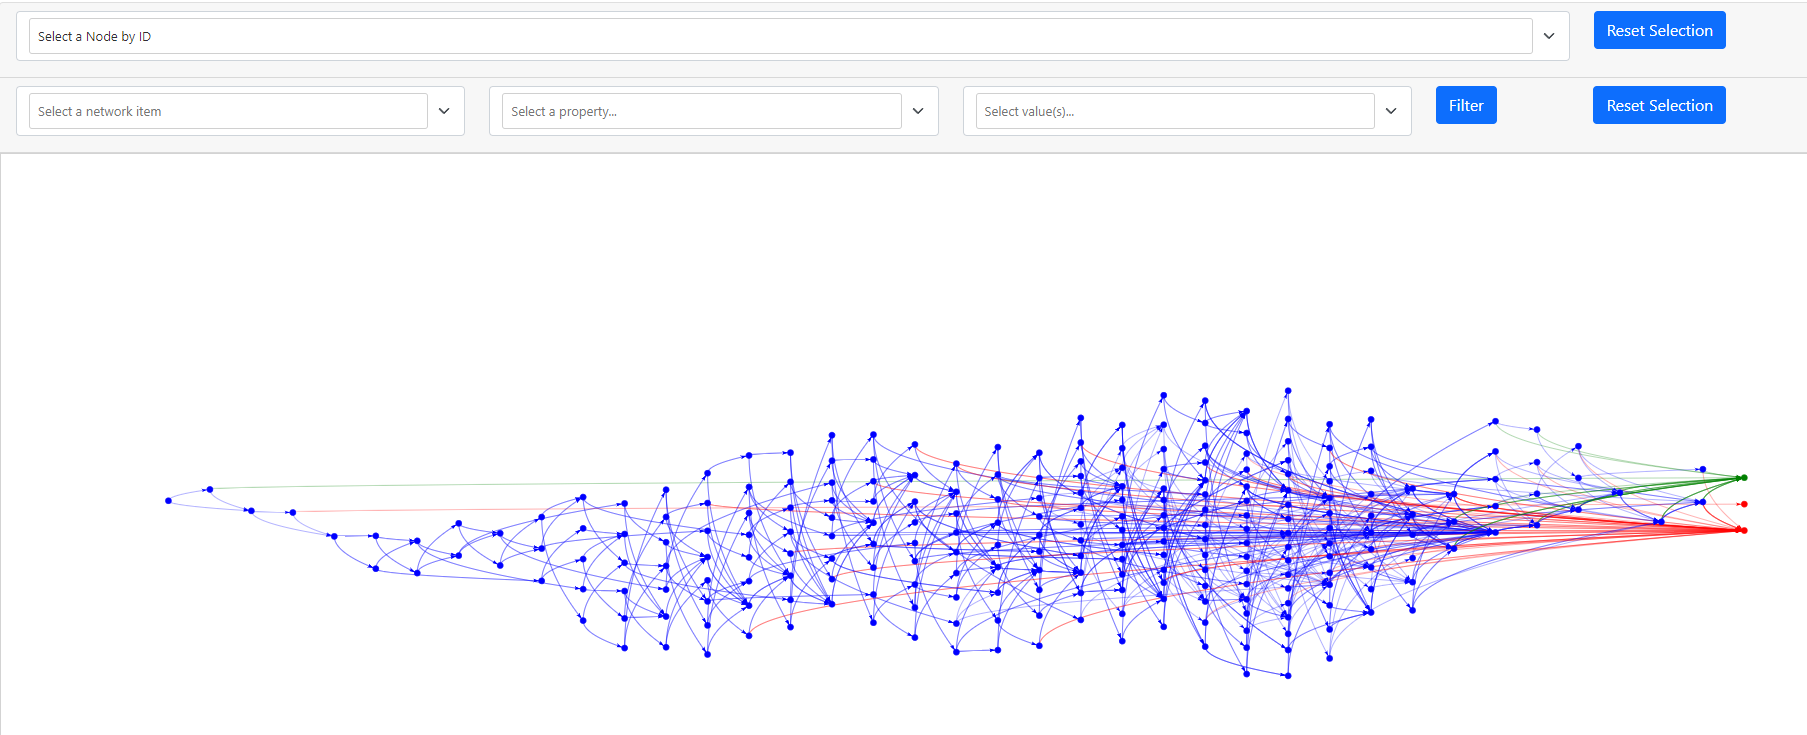
\includegraphics[scale=0.42]{visualization/overview}

States, as well as transitions leading into them, are color coded as follows:

\begin{itemize}
  \item
  The green state denotes the \texttt{Fulfilled} state, ie the one where
  there are no active rules and the contract is not breached.

  \item
  \texttt{Active} states with a nonempty set of active rules are colored blue.

  \item
  \texttt{Breached} states are colored red.
\end{itemize}

Zooming in on the start of the contract, we see that transitions are labelled
with events which are either actions,
eg \texttt{'Borrower does 'request`funds'},
or tick transitions labelled \texttt{1 day}.

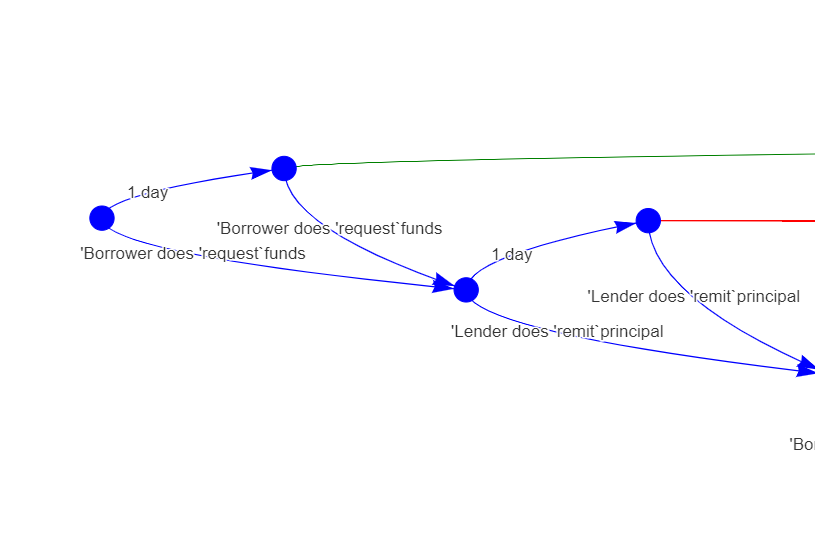
\includegraphics[scale=0.5]{visualization/zoom_start_of_contract}

Hovering over each state reveals more details about it, like the active rule
instances in an active state.
For instance, hovering over the initial state, ie the leftmost blue dot,
yields the following:

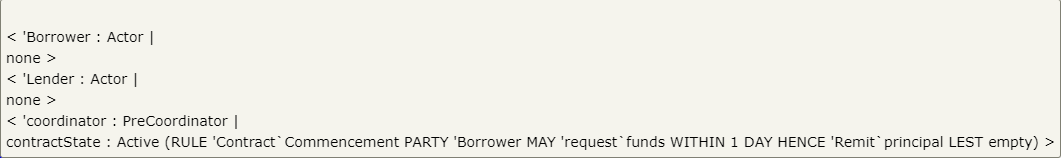
\includegraphics[scale=0.5]{visualization/initial_state}

Note that as mentioned in the previous section, states encode more metadata
than what we presented there.
These include the actors in the contract, which in this case are the
\texttt{Borrower} and \texttt{Lender}.
The state of the contract is \texttt{Active}, with the
\texttt{Contract Commencement} rule being active with an initial timer of
\texttt{1 DAY}, corresponding to its deadline.
Note that since the deadline of the rule is expressed using the \texttt{WITHIN}
keyword instead of \texttt{ON}, the borrower is allowed to request for
funds now or after 1 day.

If one day passes, the Maude implementation uses the \texttt{deltaTick}
transition function to compute the next state by decrementing the timer value
of the \texttt{Contract Commencement} active rule instance to \texttt{0 DAY}.

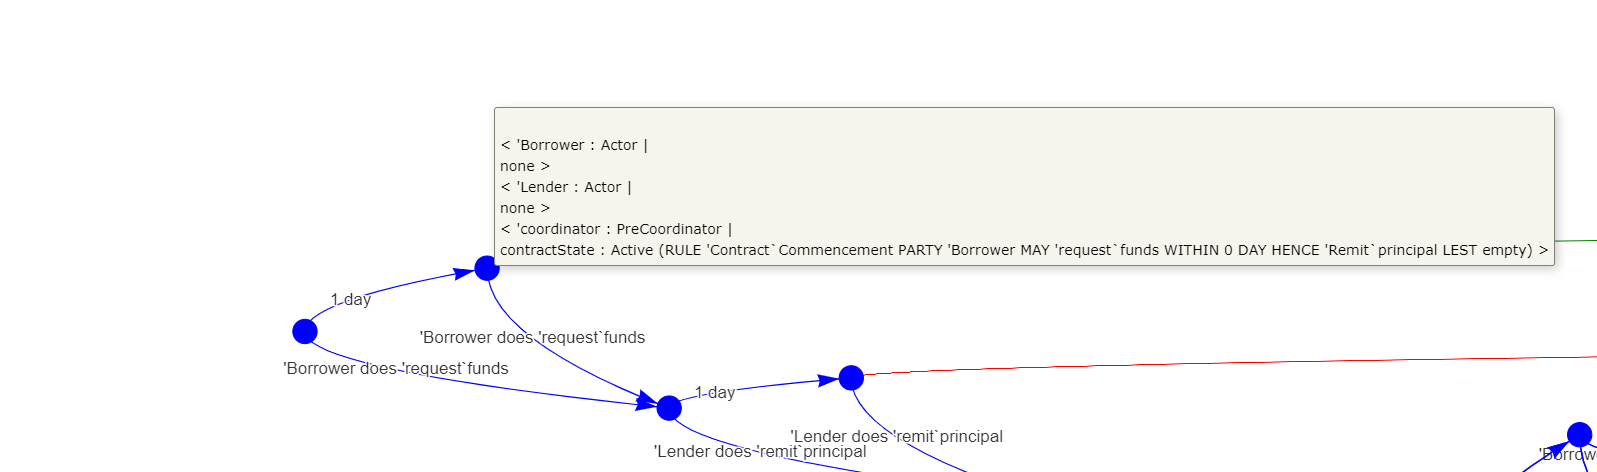
\includegraphics[scale=0.4]{visualization/initial_state_1_day_passes}

If another day passes so that the permission expires, and the borrower still
does not request for the principal, the \texttt{deltaTick} function is again
called, yielding the green \texttt{Fulfilled} state.
This is because the permission does not have a \texttt{LEST} clause, and so
no new rules are triggered once the deadline passes.

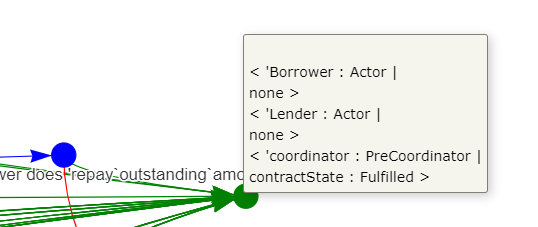
\includegraphics[scale=0.4]{visualization/fulfilled_state}

If instead, the permission is exercised, then \texttt{deltaAction} computes
the effect of that action on the current state, which is to trigger the
\texttt{HENCE} clause, ie the \texttt{Remit principal} rule.
This leads us to a state in which the lender is obliged to send the principal
amount within a day.

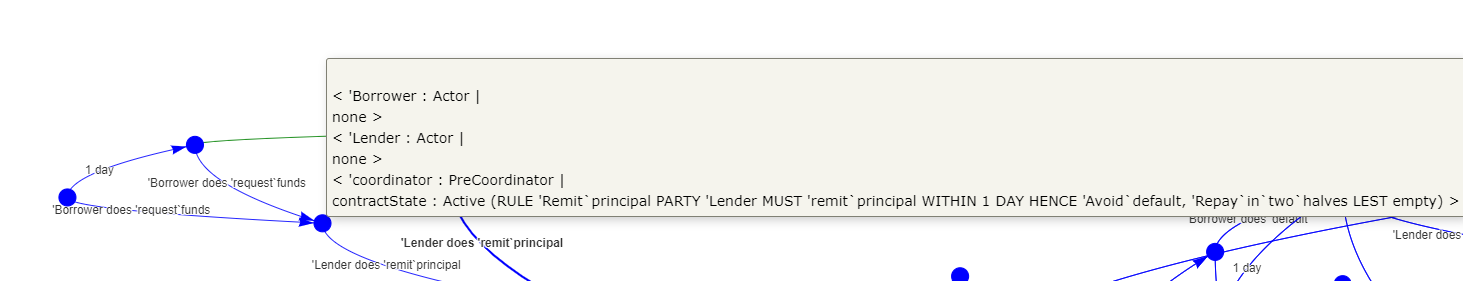
\includegraphics[scale=0.4]{visualization/state_lender_must_remit_principal}

If 2 days pass without the lender sending the principal amount,
\texttt{deltaTick} computes the resulting state to be a red breach state, with
the lender being the one to blame.

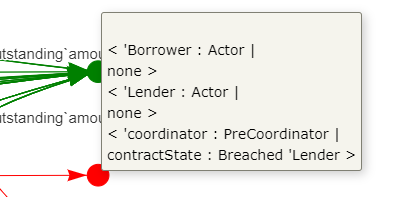
\includegraphics[scale=0.4]{visualization/state_lender_breach}

Otherwise, the action occurs and \texttt{deltaAction} triggers the
\texttt{HENCE} clause, resulting in 2
active rule instances, one prohibiting the borrower from defaulting,
and another obliging him to pay the first half.
These have an initial timer of 20 and 10 days respectively, as per their
deadlines.

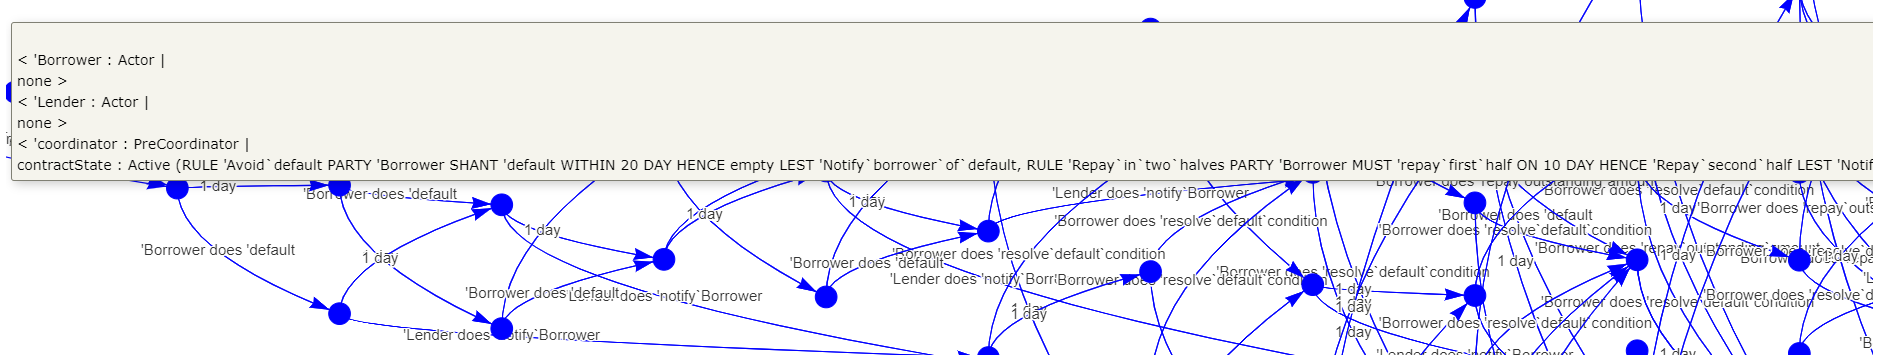
\includegraphics[scale=0.4]{visualization/state_after_sending_principal}

% \subsection{Analyzing via model checking}
% Here we should mention that in \cite{temporal_logic_norms_guido}, the author
% highlights an issue with using temporal logic to reason about deontics like
% obligations.
% We sidestep that issue due to the way we define rules as wrappers around
% events, and deontics, so that the violation of a rule corresponds directly to
% whether that event occured or not.

% For instance, a rule of the form ``Party P must do A by D'' is an obligation
% that is violated if P does not perform A by the deadline D.
% In this way, we can reason about the violation of obligations by using
% temporal logic to talk about whether an event occurred or not.

% \section{Related work}

\section{Limitations and future work}

Various shortcomings have been already mentioned in earlier sections, but
there are still others that we should mention.

Firstly, one may notice that the generated DFA is rather large, with over 100
states.
This is in spite of the fact that the loan agreement is a small contract,
with our encoding only containing rather short deadlines, ranging
up to 20 days.
One of the main reasons is our naive approach to time which we opted for due to
its simplicity.
Recall that configurations (ie states) our state space keep track of timers
that count down one day at a time as \texttt{tick} transitions occur.
This means that an active rule instance arising from a rule with a large deadline
like 365 days, can attain any value from 0 to 365 during the execution of the
contract.
Thus, the introduction of such a rule increases the number of possible states
by at least 366, growing exponentially with the number of rules and possible
timer values in the contract.

Unfortunately, this considerably bloats up the state space.
Again it must be emphasized that this is a proof of concept and these were
designed to be as high-level and close to the syntax of L4 as possible.
In the future, we intend to optimize this, among other things.

% We could investigate the use of other formalisms that better support modeling
% time and deadlines, or we could build our own abstractions to handle these more
% efficiently in Maude.

% Another shortcoming is that
% Currently, we don't yet support global variables and more sophisticated control
% structures like loops.
% Global variables would be useful to capture the notion of the outstanding amount
% in the loan agreement contract, which would then vary with the payments made by
% the borrower.
% Maude as a formalism supports these, but we currently do not support them in L4.
% For future work, we would like to provide syntax for these in L4 and translate
% them to Maude.

Perhaps the biggest downside is that while we have primarily focused our efforts
on the moving parts of a contract, ie regulative rules, we have yet to consider
static decision logic, ie constitutive rules.
What we would like to do is to allow users to define constitutive rules
and use them as ``if conditions'' in regulative rules, so that they can
write rules of the form:

\begin{lstlisting}
  RULE ruleName
  PARTY actor
  IF condition
  MUST DO action
  WITHIN n DAY
\end{lstlisting}

where the rule is only triggered if \texttt{condition} holds.

\section{Conclusions}

This paper has presented a first attempt at equipping regulative rules in L4
with an operational semantics.
In doing so, we have identified the key domain concepts in these rules and
opted for a timed transition system semantics.
We then showed how this can be implemented in Maude so that we can execute
contracts in L4 and visualize their state spaces.
Along the way, we discussed some shortcomings like how large state spaces arise
from our naive treatment of time.

While our approach has several shortcomings and is unable to fully capture
the loan agreement, we must emphasize that this is an initial attempt which
we hope to improve upon going forward.

\newpage

% Maudeibliography stuff.
\bibliographystyle{acm}
\bibliography{refs}

\end{document}